%% GENERIC STYLE SETTINGS
\usetheme{default}
\usepackage{listings}
\usepackage{multirow}
\usepackage{xcolor}

\usebackgroundtemplate{

\includegraphics[width=\paperwidth,height=\paperheight]{images/hutton_background}
}
%% PRESENTATION CONFIGURATION PARAMETERS %%%%%%%%%%%%%%%%%%%%%%%%%%%%%%%%%%%%%%%
%\titlebackgroundfile{images/hutton_title}
%\framebackgroundfile{images/hutton_background}
\definecolor{hutton_green}{HTML}{78A22F}
\definecolor{hutton_purple}{HTML}{872175}
\definecolor{hutton_blue}{HTML}{569BBE}
\usefonttheme{structurebold}
\setbeamercolor{alerted text}{fg=orange}
\setbeamercolor{background canvas}{bg=white}
\setbeamercolor{block title}{bg=hutton_purple}
\setbeamercolor{frametitle}{fg=hutton_purple}
\setbeamercolor{title}{fg=black}
\setbeamercolor{titlelike}{fg=hutton_green}
\setbeamercolor{author}{fg=hutton_purple}
\setbeamercolor{author in head/foot}{fg=white}
\setbeamercolor{title in head/foot}{fg=white}
\setbeamercolor{section in head/foot}{fg=hutton_purple}
\setbeamercolor{normal text}{fg=black}
\setbeamercolor{frametitle}{fg=hutton_purple}
\setbeamerfont{block title}{size={}}
\setbeamerfont{author}{size=\footnotesize}
\setbeamerfont{date}{size=\footnotesize}
\setbeamercolor{section in toc shaded}{fg=hutton_purple}
\setbeamercolor{section in toc}{fg=hutton_purple}
\setbeamercolor{subsection in toc shaded}{fg=hutton_purple}
\setbeamercolor{subsection in toc}{fg=hutton_purple}
\setbeamertemplate{itemize item}[circle]
\setbeamertemplate{itemize subitem}[circle]
\setbeamertemplate{itemize subsubitem}[circle]
\setbeamertemplate{itemize subsubsubitem}[circle]
\setbeamercolor{itemize item}{fg=hutton_purple}
\setbeamercolor{itemize subitem}{fg=hutton_purple}
\setbeamercolor{itemize subsubitem}{fg=hutton_purple}
\setbeamercolor{itemize subsubsubitem}{fg=hutton_purple}
\setbeamercolor{enumerate item}{fg=hutton_purple}
\setbeamercolor{enumerate subitem}{fg=hutton_purple}
\setbeamercolor{enumerate subsubitem}{fg=hutton_purple}
\setbeamercolor{enumerate subsubsubitem}{fg=hutton_purple}
\setbeamercolor{alerted text}{fg=hutton_green}
\setbeamerfont{alerted text}{series=\bfseries}
% This command makes sure that acrobat reader doesn't change the colours of the slide
% when there are figures with transparencies.
\pdfpageattr {/Group << /S /Transparency /I true /CS /DeviceRGB>>}

%Disables discrete bottom navigation bar
%\beamertemplatenavigationsymbolsempty

% Modify the slide titles to avoid the corner images,
\setbeamertemplate{frametitle}
{
\vspace{0.05\textheight}
\noindent\quad\begin{minipage}[t][0.12\textheight][t]{0.85\textwidth}
\insertframetitle\par
\end{minipage}
}

% Modify title page to avoid the big logo on right
\setbeamertemplate{title page}{
    \begin{picture}(0,0)
            %This ends up on top of the default background image, rather than replacing it:
            \put(-30,-165){%
                
\includegraphics[width=\paperwidth,height=\paperheight]{images/hutton_title}
            }
            \put(0,-75){%
                \begin{minipage}[b][0.4\textheight][t]{0.75\textwidth}
                    \usebeamerfont{title}\usebeamercolor[fg]{title}{\inserttitle\par}
                    \usebeamerfont{subtitle}\usebeamercolor[fg]{subtitle}{\insertsubtitle\par}
                \end{minipage}
            }
            \put(0,-135){%
                \begin{minipage}[b][0.1\textheight][t]{\textwidth}
                    \usebeamerfont{author}\usebeamercolor[fg]{author}{\insertauthor\par}
                \end{minipage}
            }
    \end{picture}
}

%%%%%%%%%%%%%%%%%%%%%%%%%%%%%%%%%%%%%%%%%%%%%%%%%%%%%%%%%%%%%%%%%%%%%%%%%%%%%%%%

% LISTINGS SETTING
% Settings for code listings in lstlistings

\definecolor{hutton_lightgreen}{HTML}{C8F27F}

\lstset{ %
  backgroundcolor=\color{hutton_lightgreen},   % choose the background color; you must add \usepackage{color} or \usepackage{xcolor}
  basicstyle=\tiny\ttfamily,        % the size of the fonts that are used for the code
  breakatwhitespace=true,          % sets if automatic breaks should only happen at whitespace
  breaklines=true,                 % sets automatic line breaking
  captionpos=b,                    % sets the caption-position to bottom
  commentstyle=\color{red},    % comment style
  deletekeywords={...},            % if you want to delete keywords from the given language
  escapeinside={\%*}{*)},          % if you want to add LaTeX within your code
  extendedchars=true,              % lets you use non-ASCII characters; for 8-bits encodings only, does not work with UTF-8
  frame=single,                    % adds a frame around the code
  keepspaces=true,                 % keeps spaces in text, useful for keeping indentation of code (possibly needs columns=flexible)
  keywordstyle=\color{blue},       % keyword style
%  language=Octave,                 % the language of the code
  morekeywords={*,...},            % if you want to add more keywords to the set
  numbers=left,                    % where to put the line-numbers; possible values are (none, left, right)
  numbersep=5pt,                   % how far the line-numbers are from the code
  numberstyle=\tiny\color{gray}, % the style that is used for the line-numbers
  rulecolor=\color{black},         % if not set, the frame-color may be changed on line-breaks within not-black text (e.g. comments (green here))
  showspaces=false,                % show spaces everywhere adding particular underscores; it overrides 'showstringspaces'
  showstringspaces=false,          % underline spaces within strings only
  showtabs=false,                  % show tabs within strings adding particular underscores
  stepnumber=1,                    % the step between two line-numbers. If it's 1, each line will be numbered
  stringstyle=\color{violet},     % string literal style
  tabsize=4,                       % sets default tabsize to 2 spaces
  title=\lstname                   % show the filename of files included with \lstinputlisting; also try caption instead of title
}

% Misc packages
\usepackage{multicol}

%%%
% TITLE PREAMBLE
\title[Biopython Project Update 2019] % (optional, only for long titles)
{Biopython Project Update 2019}
\subtitle{Standing on each other's shoulders \\ 
\includegraphics[height=3cm]{images/biopython_logo_m.png}}
\author[Cock] % (optional, for multiple authors)
{Peter~Cock (\href{https://twitter.com/pjacock}{@pjacock on Twitter}), \\
The Biopython Contributors (\href{https://twitter.com/Biopython}{@biopython on Twitter})}
\institute[The James Hutton Institute] % (optional)
{
  Information and Computational Sciences\\
  The James Hutton Institute
}
\date[July 2019] % (optional)
{Basel, Switzerland, 25$^{th}$ July 2019}
\subject{Bioinformatics}

%%%
% START DOCUMENT
\begin{document}

\frame[plain]{\titlepage}

\begin{frame}
\frametitle{Contents}
\begin{itemize}
\item Introducing Biopython
\item Contributors and releases this past year
\item Dual licensing update
\item Documentation and automation
\item On going and planned work
\item Community building
\end{itemize}
\end{frame}

\begin{frame}
  \frametitle{What is Biopython?}

  \begin{itemize}
  \item Collection of modules for biological computation in Python
  \begin{itemize}
  \item Sequence handling and motifs, parsers, database queries, protein structures, phylogenetics, tool wrappers and more.
  \end{itemize}
  \item Started in 1999, first release in 2000
  \item Open source and freely available (Biopython license)
  \item \url{https://biopython.org} and @Biopython on Twitter
  \end{itemize}

\center

\includegraphics[height=2.5cm]{images/biopython_logo_m.png}
\end{frame}


\begin{frame}
  \frametitle{38 named contributors in last year, \\ 16 newcomers with star!}
  \scriptsize{
  \begin{multicols}{3}
  \begin{itemize}
    \item Alona Levy-Jurgenson*
    \item Andrey Raspopov*
    \item Antony Lee
    \item Ariel Aptekmann
    \item Benjamin Rowell*
    \item Bernhard Thiel
    \item Brandon Invergo
    \item Catherine Lesuisse
    \item Chris Rands
    \item Darcy Mason*
    \item Deepak Khatri*
    \item Devang Thakkar*
    \item Gert Hulselmans
    \item Ivan Antonov*
    \item Jared Andrews
    \item Jens Thomas*
    \item Jeremy LaBarage*
    \item Juraj Szász*
    \item Kai Blin
    \item Konstantin Vdovkin*
    \item Lenna Peterson
    \item Manuel Nuno Melo*
    \item Mark Amery
    \item Markus Piotrowski
    \item Maximilian Greil
    \item Micky Yun Chan*
    \item Nick Negretti*
    \item Peter Cock
    \item Peter Kerpedjiev
    \item Ralf Stephan
    \item Rob Miller
    \item Rona Costello*
    \item Sergio Valqui
    \item Spencer Bliven
    \item Victor Lin
    \item Wibowo 'Bow' Arindrarto
    \item Yi Hsiao*
    \item Zheng Ruan
  \end{itemize}
  \end{multicols}
  }
\end{frame}


\begin{frame}
\frametitle{Recent releases}
\begin{itemize}
\item \href{https://www.open-bio.org/2018/12/18/biopython-1-73-released/}{Biopython 1.73 (April 2019)}
  \begin{itemize}
  \item Added Python 3.7 support
  \end{itemize}
\item \href{https://www.open-bio.org/2019/07/16/biopython-1-74-released/}{Biopython 1.74 (July 2019)}
  \begin{itemize}
  \item Finally have full API "docstring" coverage, \\
        special mention to recent contributor Sergio Valqui
  \end{itemize}
\item Most code changes to:
  \begin{itemize}
  \item API documentation
  \item Python coding style
    \begin{itemize}
    \item No consensus on adopting \texttt{black} Python formatting style
    \end{itemize}
  \item Dual licensing...
  \end{itemize}
\end{itemize}
\end{frame}


\begin{frame}
\frametitle{Biopython's Open Source License}
\begin{itemize}
\item Open Source Initiative \url{https://opensource.org/}
    maintains a list of approved open source licenses
\item Biopython's license is not (quite) on that list
\item We're gradually dual-licensing under 3-clause BSD license
\item Requires checking each file to confirm all contributors agree
\item Biopython 1.70 (July 2017), about $2\%$ of main code done
\item Biopython 1.72 (June 2018), about $30\%$ of main code done
\item Biopython 1.74 (July 2019), just over $50\%$ of main code done
\end{itemize}
\end{frame}


\begin{frame}
\frametitle{Documentation}
\begin{itemize}
\item Documentation on our main website
  \begin{itemize}
  \item Originally MediaWiki
  \item Converted to Markdown using GitHub Pages
  \end{itemize}
\item Tutorial and Cookbook
  \begin{itemize}
  \item Written in \LaTeX for PDF and HTML
  \end{itemize}
\item API documentation (Python ``docstrings'' in the code)
  \begin{itemize}
  \item Had been turned into HTML using \texttt{epydoc}
  \item Standardised on reStructuredText (RST)
  \item Now using Sphinx \texttt{apidoc}
  \end{itemize}
\end{itemize}
\end{frame}

\begin{frame}
\frametitle{Documentation - biopython.org}
\vspace{-0.8cm}
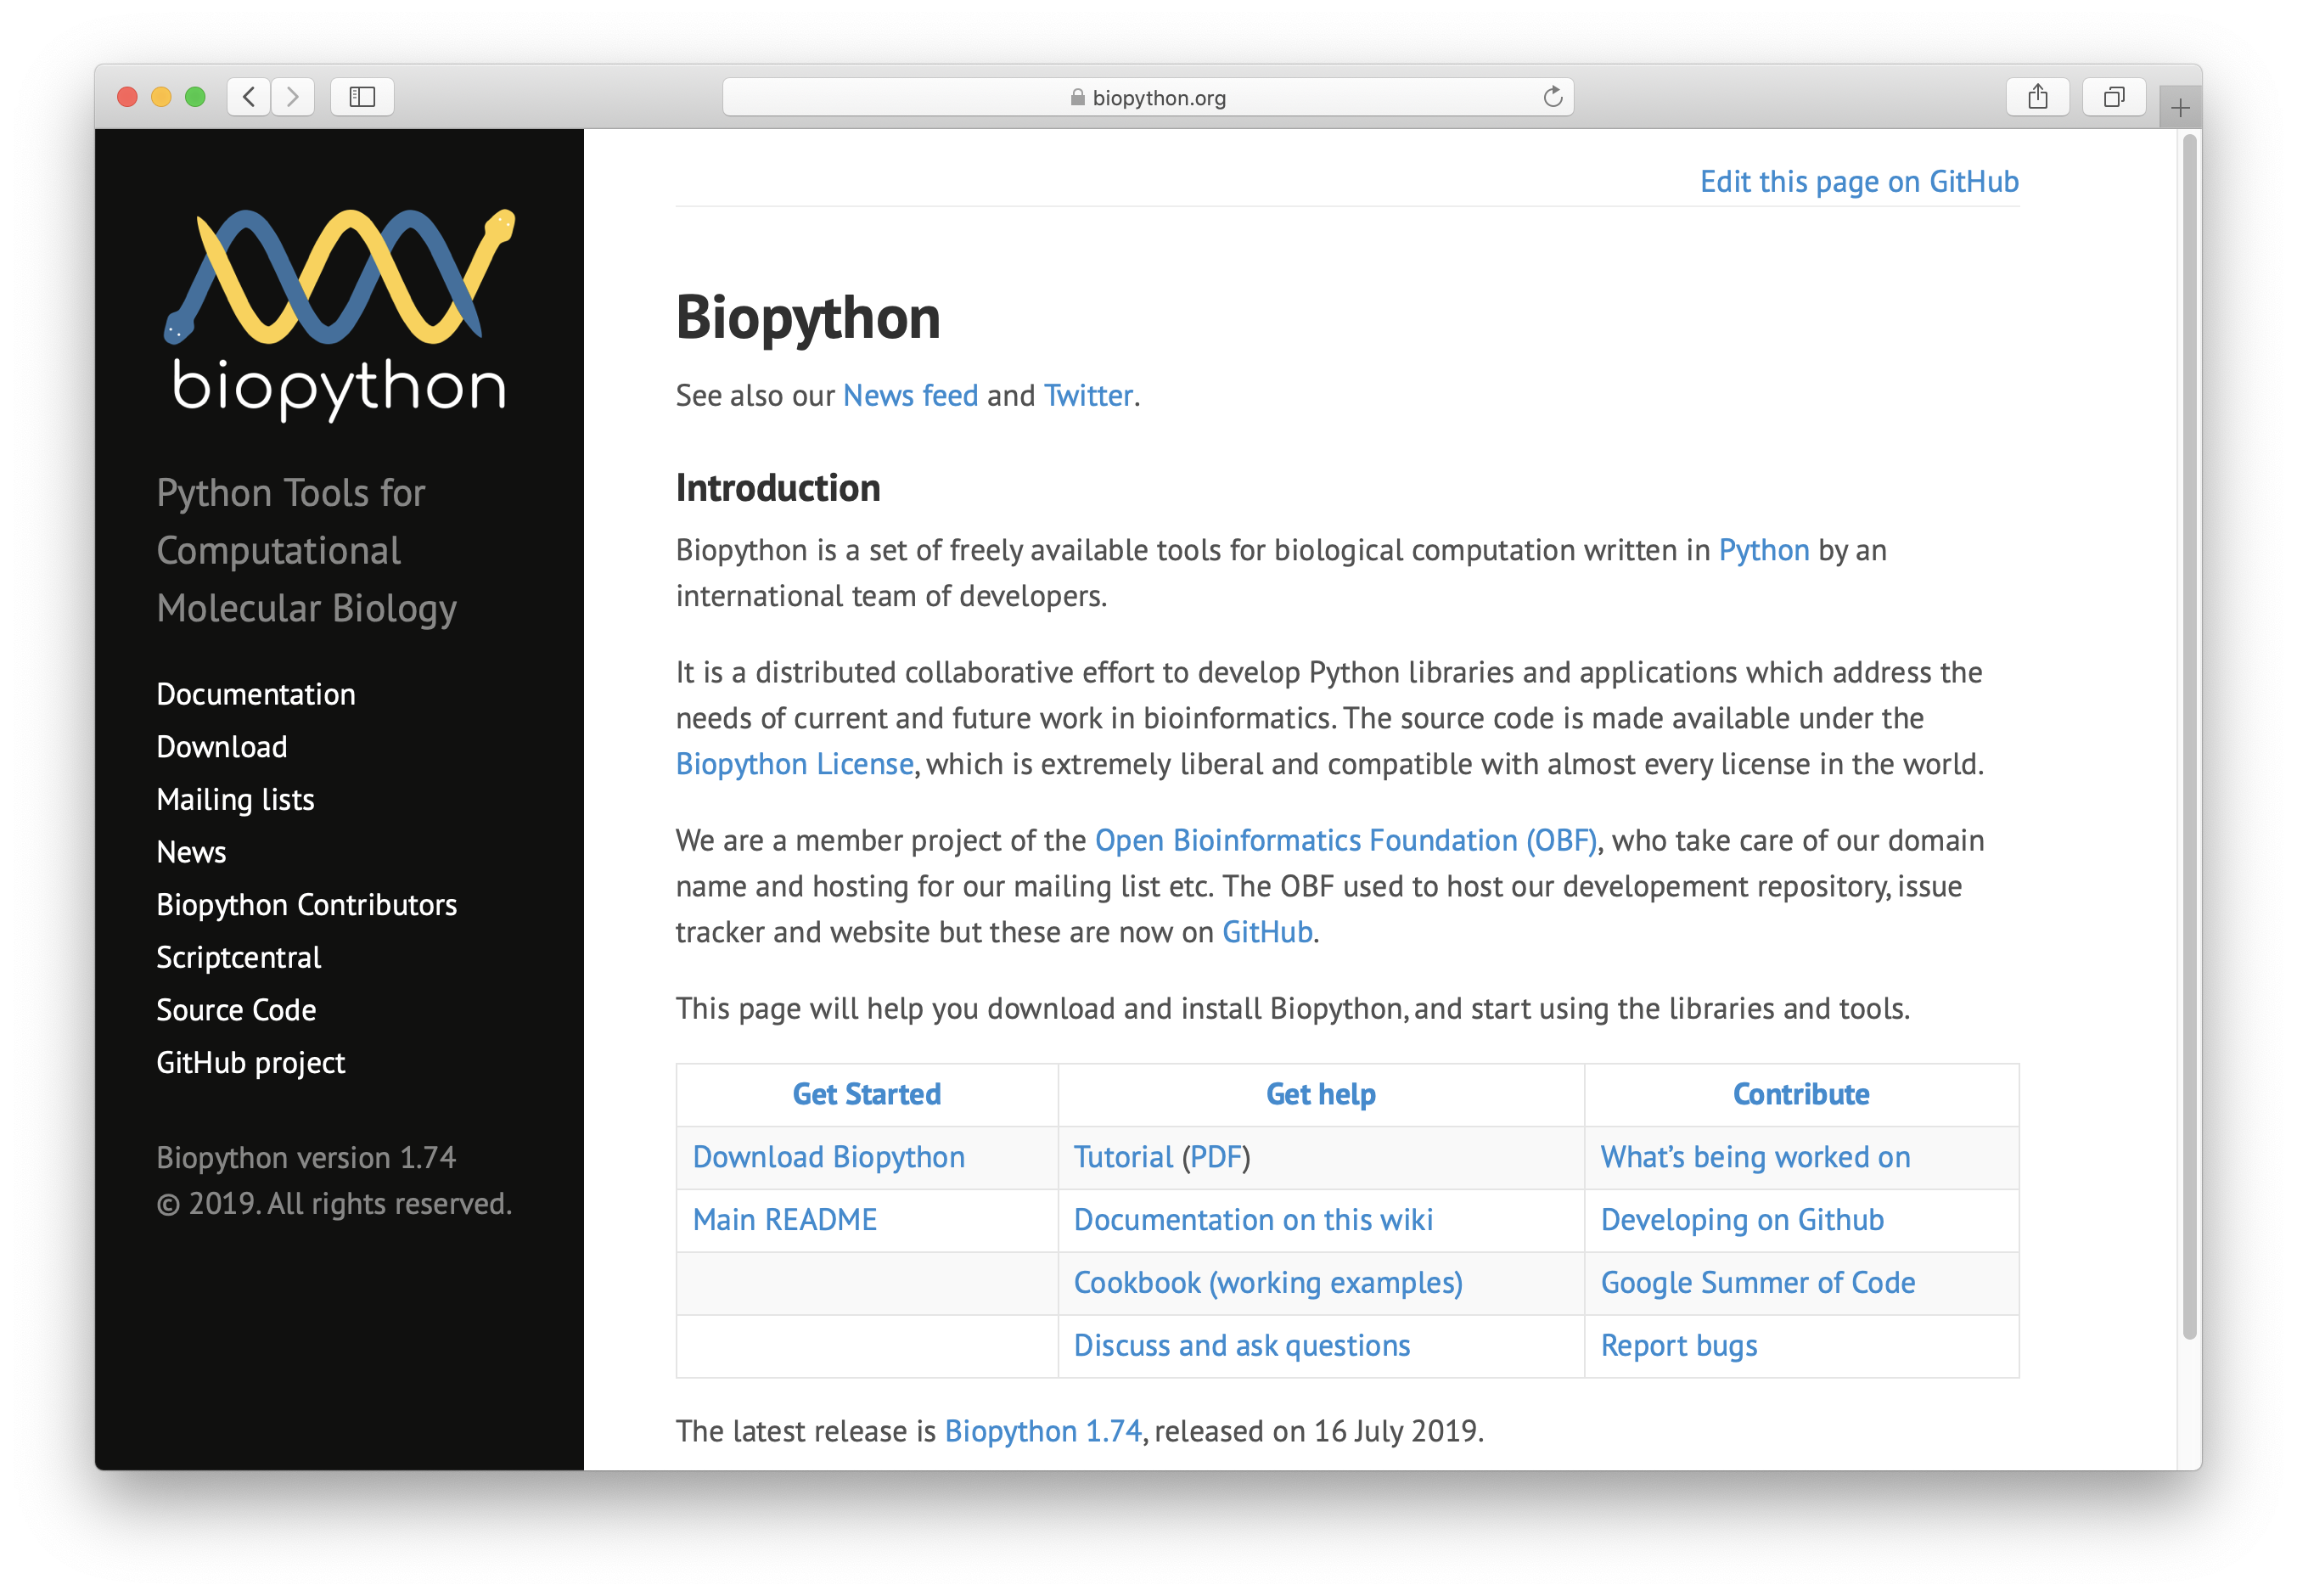
\includegraphics[width=\textwidth]{images/main}
\end{frame}

\begin{frame}
\frametitle{Documentation - API via epydoc (old)}
\vspace{-0.8cm}
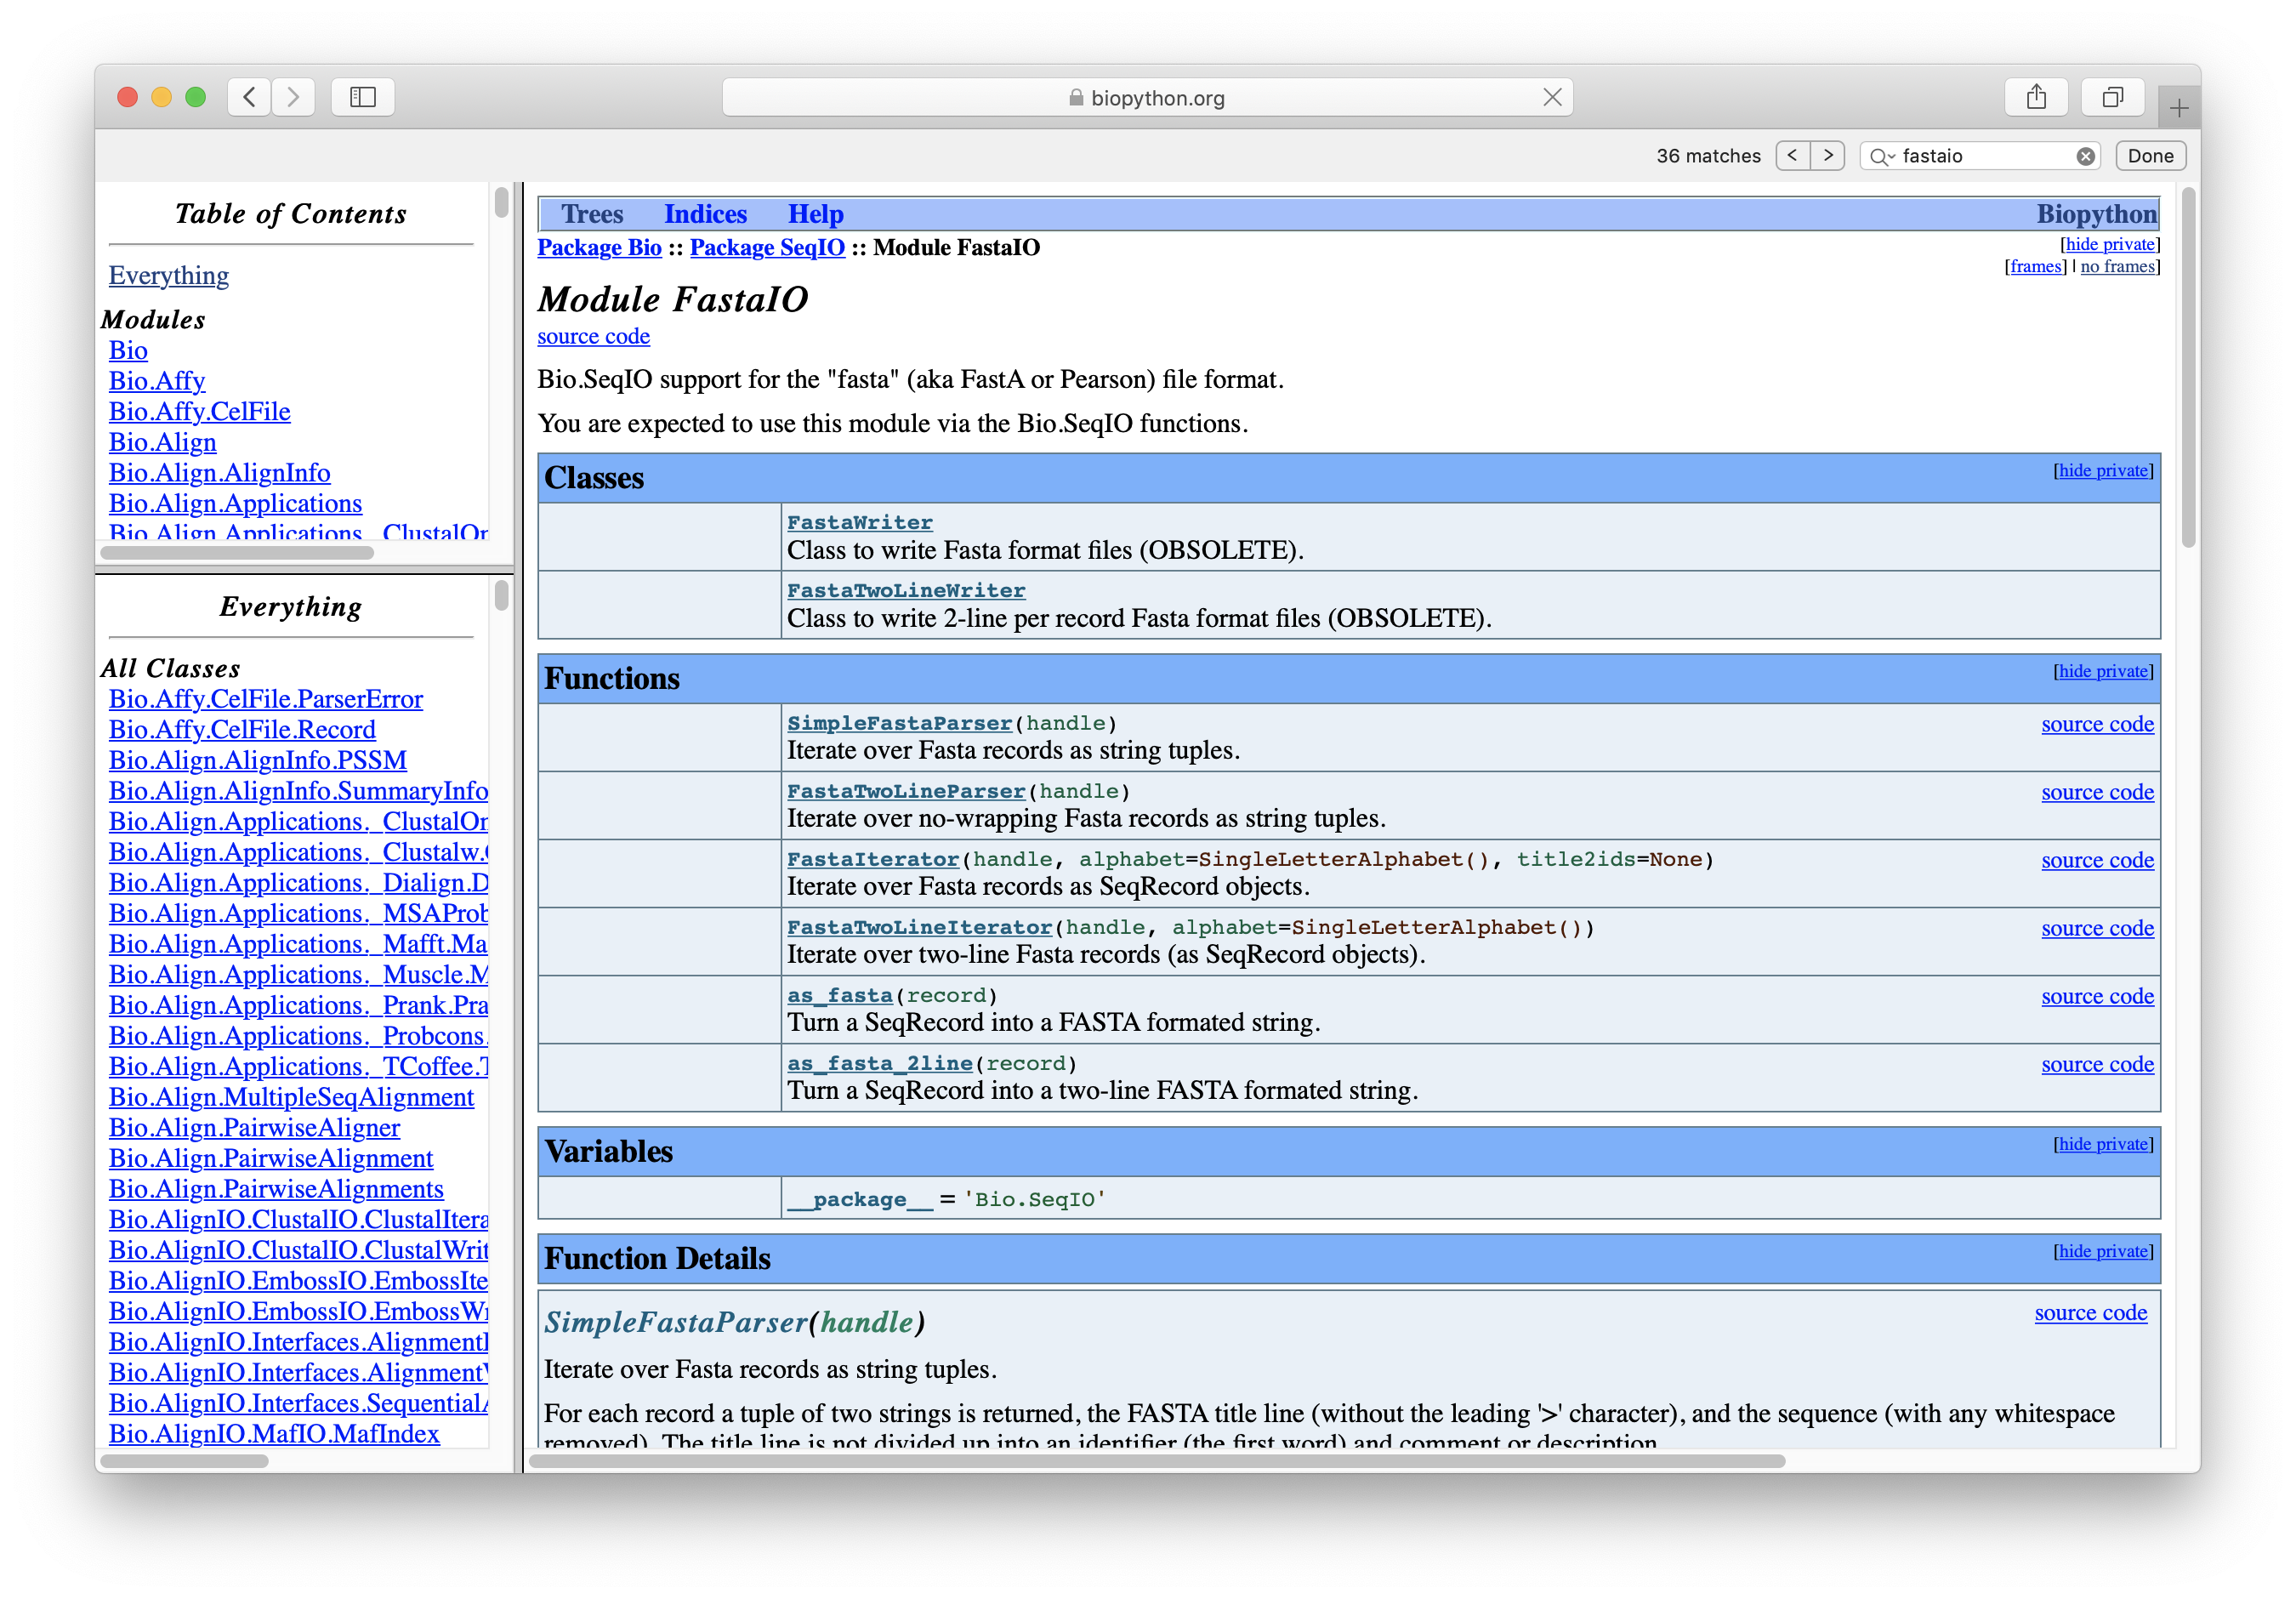
\includegraphics[width=\textwidth]{images/epydoc}
\end{frame}

\begin{frame}
\frametitle{Documentation - API via Sphinx apidoc}
\vspace{-0.8cm}
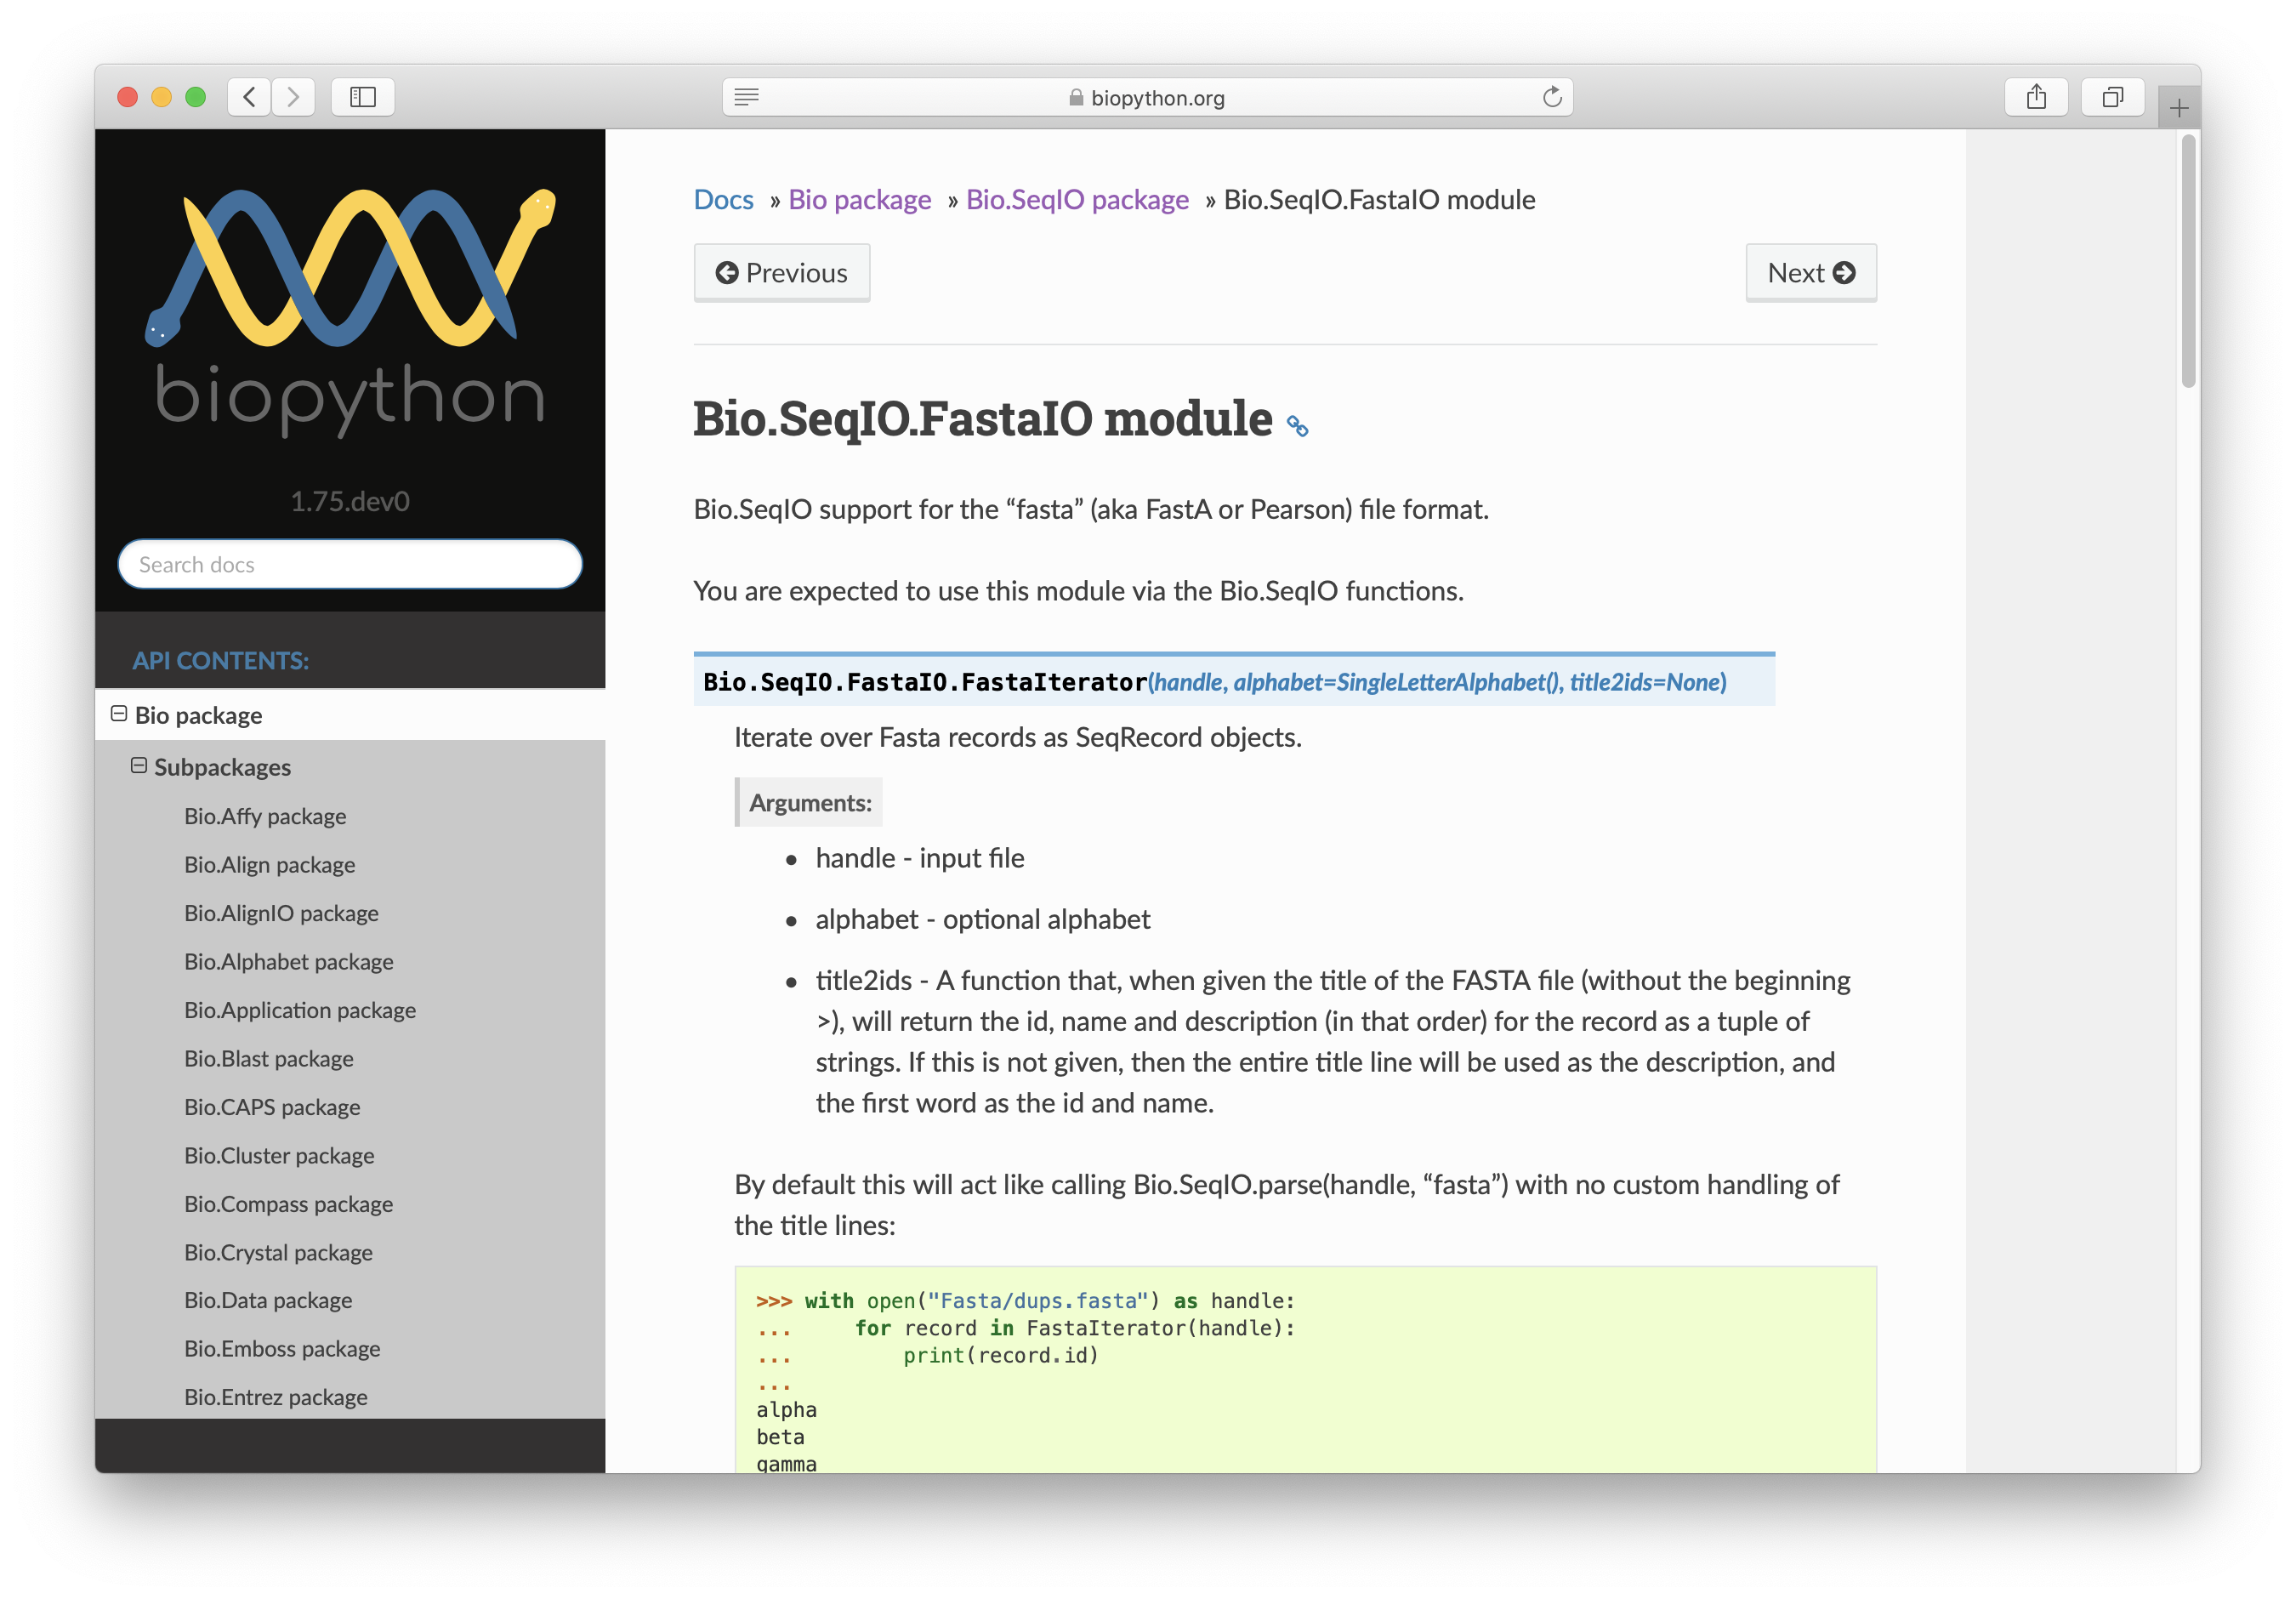
\includegraphics[width=\textwidth]{images/sphinx-apidoc}
\end{frame}

\begin{frame}
\frametitle{In progress: Tutorial \textit{\&} API via Sphinx?}
\vspace{-0.8cm}
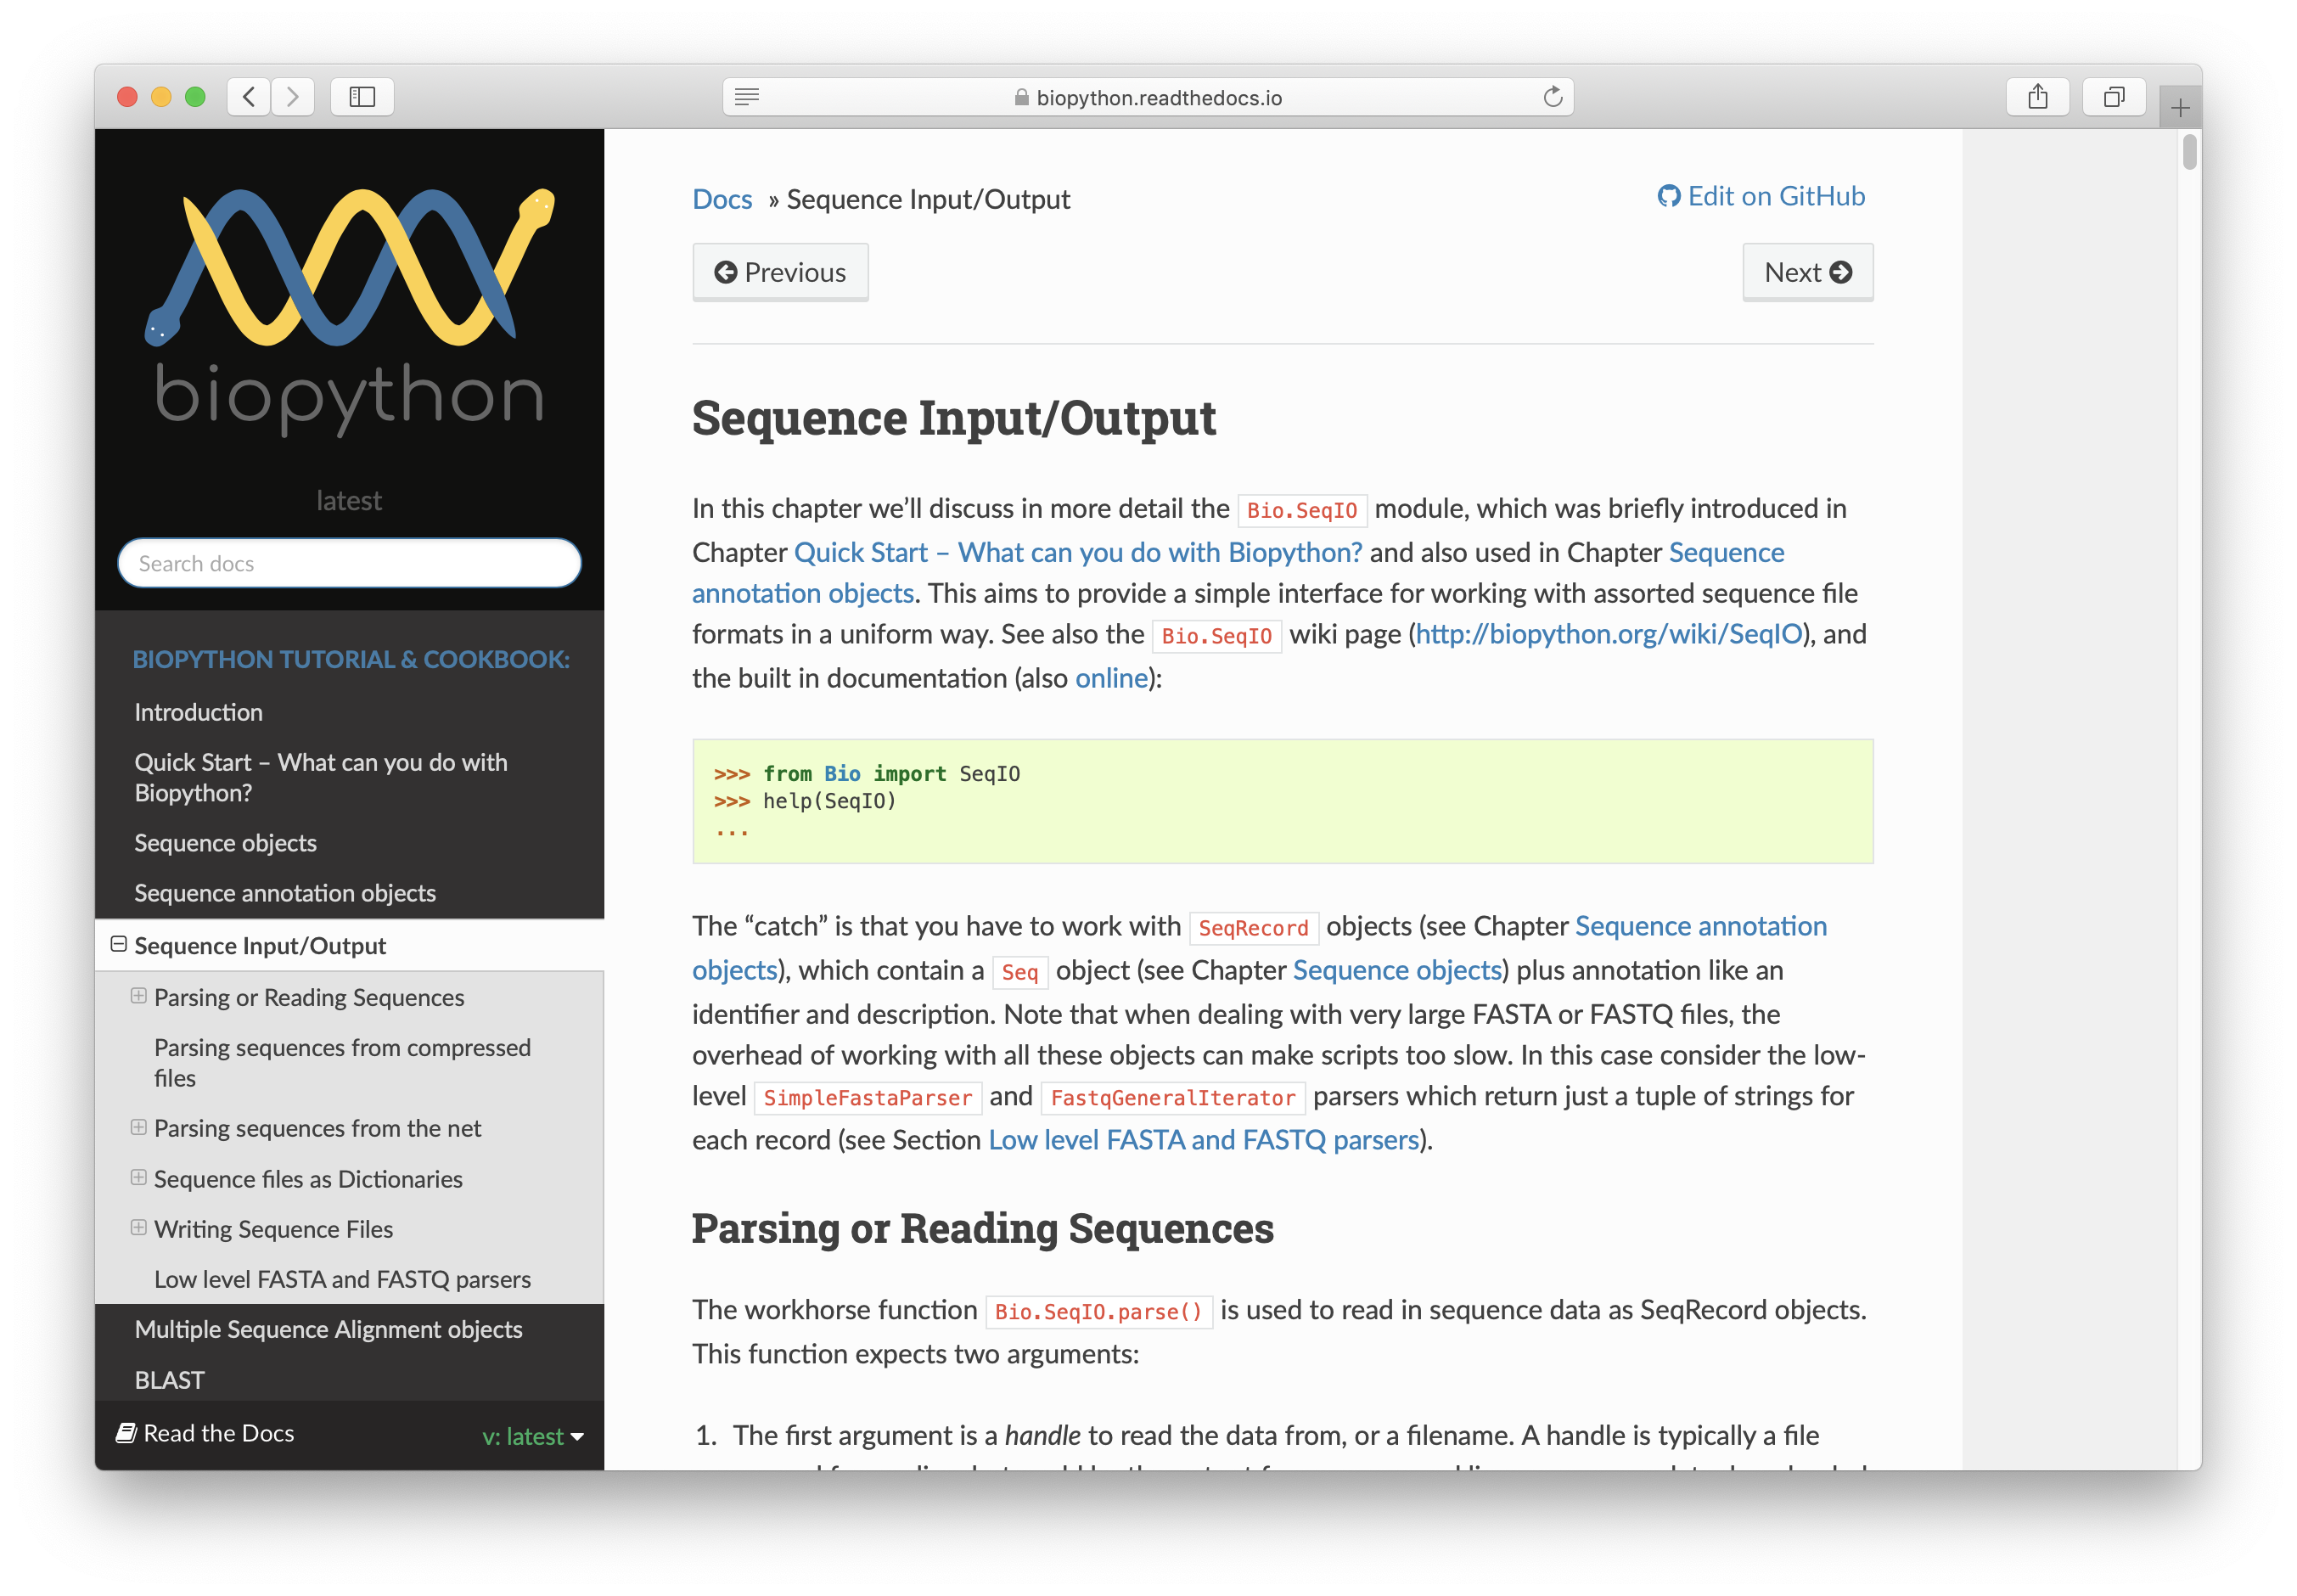
\includegraphics[width=\textwidth]{images/read-the-docs}
\end{frame}

\begin{frame}
\frametitle{Documentation - Automation}
\begin{itemize}
\item Website - automatic publishing on GitHub pages
\item Tutorial \& cookbook - manual step for each release
\item Running \texttt{epydoc} was manual step for each release
\item Running Sphinx \texttt{apidoc} under TravisCI
  \begin{itemize}
  \item Deploying Sphinx \texttt{apidoc} via GitHub Pages
  \item Automatic destination based on version, e.g.
    \begin{itemize}
    \item \url{https://biopython.org/docs/1.74/api/}
    \item \url{https://biopython.org/docs/dev/api/}
    \end{itemize}
  \end{itemize}
\item Next steps
  \begin{itemize}
  \item Fine tune Sphinx \texttt{apidoc} presentation
  \item Better match Sphinx and website themes
  \item Automate Tutorial \& Cookbook build and deploy
  \end{itemize}
\end{itemize}
\end{frame}

\begin{frame}
\frametitle{Release builds - Automation}
\begin{itemize}
\item Build pre-compiled wheels on AppVeyor \& TravisCI
    \begin{itemize}
        \item Following NumPy community in using the multibuild system, \\
              developed by Matthew Brett and the MacPython project. \\
              \url{https://github.com/matthew-brett/multibuild} \\
              \url{https://github.com/biopython/biopython-wheels}
    \end{itemize}
\item Uploaded to Python Package Index (PyPI)
\item Recommend \texttt{pip install biopython}
\item Thanks to conda-forge, can do \texttt{conda install biopython}
\end{itemize}
\end{frame}


\begin{frame}
\frametitle{Python Versions - Testing Automation}
\begin{itemize}
\item Currently test on Python 2.7, 3.4, 3.5, 3.6, and 3.7
\item About to drop Python 3.4 and add Python 3.8
\item Clear end of life for Python 2 support in 2020, \\ we've pledged on \url{http://python3statement.org/}
\item Also support and test on PyPy
\item Support for Jython deprecated
\end{itemize}
\end{frame}


\begin{frame}
\frametitle{On going and planned work}
\begin{itemize}
    \item Further simplify release \& documentation builds
    \item Improving compliance with PEP8 and PEP257 style guidelines
    \item Start working towards \texttt{numpydoc} style for docstrings?
    \item Improving code test coverage \url{https://codecov.io/github/biopython/biopython/}
    \item Removing/simplifying  legacy Alphabet objects
    \item Dropping Python 2 support in early 2020 (see above)
    \item Other contributor driven efforts
\end{itemize}
\end{frame}


\begin{frame}
\frametitle{Changes to help Community Building}
\begin{itemize}
\item Already use:
   \begin{itemize}
   \item GitHub Issue templates (helps bug reporting)
   \item GitHub Pull Request templates (to help with expectations)
   \item \textit{Easy Fix} tag on some issues, intended for new contributors
   \item \texttt{CONTRIBUTING} file highlighting coding conventions etc
   \item \texttt{CODEOWNERS} file to help assign code reviews
   \end{itemize}
\item Discussing an OBF-wide \textit{Code of Conduct}
\item \textbf{What else should we be doing?}
\end{itemize}
\end{frame}


\begin{frame}
\frametitle{Acknowledgements}
Thank you to:
\begin{itemize}
    \item All our contributors to date
    \item Contributors' funders for indirect support
    \item Google Summer of Code (supporting past students)
    \item Open Bioinformatics Foundation (OBF) for domain name, mailing lists, etc -- any maybe later a Code of Conduct?
\end{itemize}

\vspace{1.1cm}
\center
\includegraphics[width=0.9\paperwidth]{../images/Hutton-thanks-banner}
\end{frame}

% etc
\end{document}
